% در این قسمت نحوه‌ی نصب بر روی سیستم عامل اوپن سوزی شرح داده می شود. به دلیل اینکه در اوپن سوزی
% روشی ساده با گرافیکی کاربرپسند برای نصب برنامه ها وجود دارد، نصب روی این سیستم عامل را به طور جداگانه
% علاوه بر سیستم عامل‌های لینوکسی آورده‌ایم.
% محمد هادی منصوری ۹۰/۳/۳
\section{\lr{OpenSUSE}}

اگرچه دستورالعمل مربوط به نصب \lr{Doxygen} روی سیستم عامل‌های لینوکسی برای سیستم
عامل \lr{OpenSUSE} هم قابل استفاده است، اما سیستم عامل \lr{OpenSUSE} روشی
گرافیکی ساده و کاربرپسندی برای نصب برنامه‌ها دارد.
در این سیستم عامل مدیریت گرافیکی \lr{YaST} امکانات مناسبی برای مدیریت قسمت‌های
مختلف سیستم فراهم آورده است.
از جمله‌ی این امکانات مدیریت مخزن‌ها\footnote{\lr{Repository}}و مدیریت
نرم‌افزارها\footnote{\lr{Software Management}} است.

برای نصب \lr{Doxygen}، ابتدا باید به اینترنت وصل باشید. سپس از طریق منوی شروع در
\lr{OpenSUSE} که با علامت 
\includegraphics[width=0.5cm]{image/opensuse} نشان
داده می‌شودبرنامه‌ی \lr{YaST} را اجرا کنید. سپس قسمت \lr{Software Management} را
انتخاب کنید. پس از اینکه ابزار مدیریت نرم‌افزارها باز شد، در قسمت جستجو، کلمه‌ی
\lr{doxy} را جستجو کنید. در فهرستی که از نتیجه‌ی جستجو نشان داده می‌شود
برنامه‌های \lr{doxygen} و \lr{doxywizard} را به حالت انتخاب در آورید، و سپس
دکمه‌ی تایید را بزنید تا سیستم شروع به نصب برنامه‌ها کند. هر کدام از این
برنامه‌ها که قبلا روی سیستم شما نصب شده باشند به حالت انتخاب شده هستند و نیازی
به نصب آن ندارید. البته ممکن است که بخواهید آن برنامه را به‌روز کنید. تصویر
\ref{image/install/OpenSUSE/setup} را مشاهده کنید.

\begin{figure}
 \centering
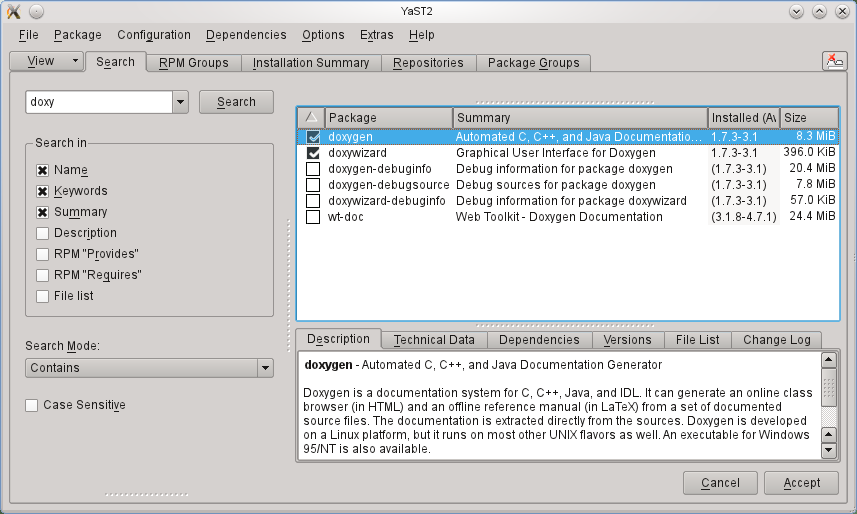
\includegraphics[width=0.75\textwidth]{image/install/OpenSUSE/setup}
\caption[پنجره‌ی نصب برنامه‌ها در سیستم عامل \lr{OpenSUSE}.]{
پنجره‌ی نصب برنامه‌ها در سیستم عامل \lr{OpenSUSE}. پس از جستجوی نام ابزار مورد
نظر خود، آن‌ها را انتخاب کرده و سپس شروع به نصب کنید.
}
\label{image/install/OpenSUSE/setup}
\end{figure}

در صورتی که \lr{doxygen} یا \lr{doxywizard} در نتایج جستجو مشاهده نشد، احتمالا
مخزن مربوط به این نرم‌افزارها در فهرست مخزن‌های سیستم شما وجود ندارد و باید آن
را اضافه کنید. برای این کار ابتدا آدرس یک مخزن که این ابراز را دارد پیدا کنید
سپس در \lr{YaST} به قسمت \lr{Software Repositories} رفته و این آدرس را به فهرست
مخزن‌های سیستم اضافه کنید. پس از آن دوباره نام ابزارها را جستجو کنید و آن‌ها را
نصب کنید.

